%----------------------------------------------------------------------------------------
%	EISCAT MADRIGAL.
%----------------------------------------------------------------------------------------

\section{EISCAT Madrigal}
In figure \ref{fig:madrigal} the EISCAT data from the 30th of October 2003 is shown. There are a few white gaps which can be explained by interference like clouds in the atmosphere. On top we have the electron density, followed by the electron temperature, ion temperature, ion drift velocity and the system temperature. \\

On the 30th of October there were some M-flares at 1:55 till 2:45 and 15:20 till 15:40 measured by GOES \cite{goes_x-ray_archive}.





\begin{figure}
\centering
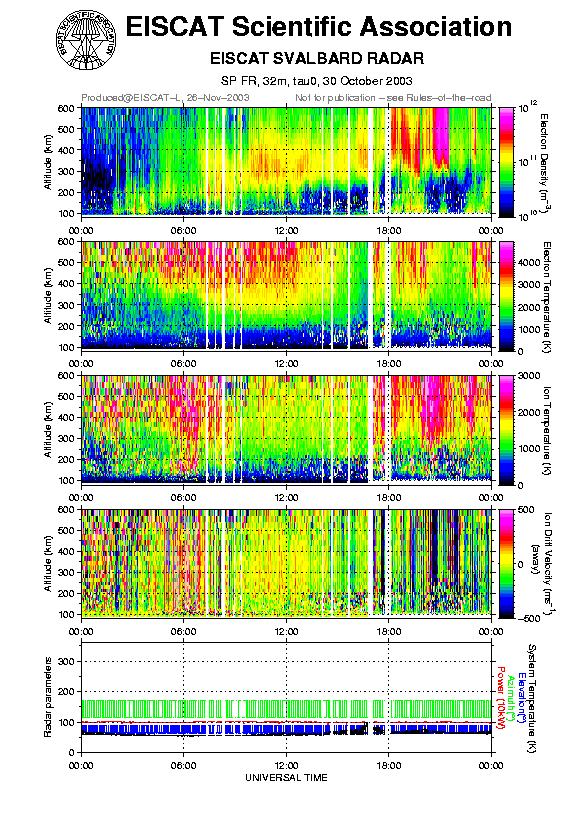
\includegraphics[width=.9\textwidth]{figures/2003-10-30_SvalvardPlot.png}
\caption{EISCAT radar data from the upper atmosphere science database Madrigal \cite{madrigal}.}
\label{fig:madrigal}
\end{figure}